
%(BEGIN_QUESTION)
% Copyright 2012, Tony R. Kuphaldt, released under the Creative Commons Attribution License (v 1.0)
% This means you may do almost anything with this work of mine, so long as you give me proper credit

The following is an electrical schematic diagram for a General Electric model IAC77 electromechanical instantaneous/time-overcurrent protective relay:

$$\includegraphics[width=15.5cm]{i01970x01.eps}$$

\vskip 10pt

Identify the following:

\begin{itemize}
\item{} What type of symbol represents a coil of wire in this schematic
\item{} What type of symbol represents a relay contact in this schematic
\item{} What type of symbol represents a resistor in this schematic
\item{} What type of symbol represents a capacitor in this schematic
\item{} Where to connect the current transformer to the relay
\item{} How to make coarse adjustments of the pick-up value for the 51 (time-overcurrent) function
\item{} How to make fine adjustments of the pick-up value for the 51 (time-overcurrent) function
\item{} How to make adjustments of the pick-up value for the 50 (instantaneous overcurrent) function
\item{} Whether or not 50 and 51 pickup adjustments are {\it interactive} (i.e. adjusting one affects the adjustment of the other)
\item{} The purpose of having a seal-in unit
\item{} How to wire the relay so it only functions as a ``50'' (instantaneous overcurrent) unit
\item{} How to wire the relay so it only functions as a ``51'' (time overcurrent) unit
\item{} How to wire the relay so it performs both ``50'' and a ``51'' protective functions
\item{} Why the circuit breaker has an auxiliary contact (52a) connected in series with the trip coil (note: this contact opens and closes simultaneously with the breaker's main power contacts, being operated by the same mechanism)
\end{itemize}

\underbar{file i01970}
%(END_QUESTION)





%(BEGIN_ANSWER)

\noindent
{\bf Partial answer:}

The pickup adjustments for the 50 function and the 51 function are non-interactive: adjusting one of them does not affect the adjustment of the other.

\vskip 10pt

The reason the breaker's trip coil is wired in series with the normally-open 52a auxiliary contact is to the trip circuit will not continue to (needlessly) draw current from the station battery power supply after the breaker has already been tripped.  Thus, the 52a contact unlatches the 51 relay's ``seal-in'' circuit once the breaker reaches the tripped position.

%(END_ANSWER)





%(BEGIN_NOTES)

$$\includegraphics[width=15.5cm]{i01970x02.eps}$$

The CT input is terminals 5 and 6.

\vskip 10pt

The coarse time-overcurrent pickup adjustment is the tapped transformer winding (primary) on the right-hand side of the diagram. 

\vskip 10pt

The fine time-overcurrent pickup adjustment is the variable resistor on the secondary side of the tapped transformer on the right-hand side of the diagram. 

\vskip 10pt

The instantaneous pickup value is adjusted by moving the core (pole) on the instantaneous unit.

\vskip 10pt

The time-overcurrent and instantenous overcurrent adjustments are non-interacting.

\vskip 10pt

The seal-in unit protects the delicate induction disk switch contacts from excessive arcing during a trip event.  As soon as trip coil current flows, the seal-in unit latches the relay on so that trip current does not get interrupted if the induction disk contacts happen to ``bounce''.

\vskip 10pt

For instantaneous trip operation only, wire trip circuit to terminals 1 and 3.

\vskip 10pt

For timed trip operation only, wire trip circuit to terminals 1 and 2.

\vskip 10pt

For either instantaneous or timed trip operation, jumper terminals 2 and 3, then wire trip circuit to terminals 1 and 2/3.

\vskip 10pt

The purpose of the 52a contact in series with the breaker trip coil is to interupt tripping circuit current as soon as the breaker opens.  Otherwise, the trip circuit would needlessly drain current from the station battery.  It would also make it difficult to re-close the breaker when needed: the relay's trip circuit would have to be manually broken to cause the seal-in unit to unlatch, before the breaker could be re-closed.



\vskip 20pt \vbox{\hrule \hbox{\strut \vrule{} {\bf Virtual Troubleshooting} \vrule} \hrule}

This question is a good candidate for a ``Virtual Troubleshooting'' exercise.  Presenting the diagram to students, you first imagine in your own mind a particular fault in the system.  Then, you present one or more symptoms of that fault (something noticeable by an operator or other user of the system).  Students then propose various diagnostic tests to perform on this system to identify the nature and location of the fault, as though they were technicians trying to troubleshoot the problem.  Your job is to tell them what the result(s) would be for each of the proposed diagnostic tests, documenting those results where all the students can see.

During and after the exercise, it is good to ask students follow-up questions such as:

\begin{itemize}
\item{} What does the result of the last diagnostic test tell you about the fault?
\item{} Suppose the results of the last diagnostic test were different.  What then would that result tell you about the fault?
\item{} Is the last diagnostic test the best one we could do?
\item{} What would be the ideal order of tests, to diagnose the problem in as few steps as possible?
\end{itemize}

\vskip 20pt \vbox{\hrule \hbox{\strut \vrule{} {\bf Virtual Trip-testing} \vrule} \hrule}

This question is a good candidate for a ``Virtual Trip-testing'' exercise.  Presenting the diagram to students, you pose an assignment whereby students must figure out how to test some component of this system to check that it will operate as intended to shut down the system in an abnormal (trip) condition, with some realistic limitation (e.g. power cannot be shut off to the load).  Students then propose various methods for executing the test.  Your job is to determine whether or not their proposed tests will achieve the desired result(s).

During and after the exercise, it is good to ask students follow-up questions such as:

\begin{itemize}
\item{} Where might our planned test strategy go wrong?  In other words, what thing(s) might happen to foil our test, either to invalidate the results or to not honor the stated limitation(s)?
\item{} Suppose the limitation were different.  How would this affect our ability to carry out the test?
\item{} Is the last test strategy best one we could execute?
\end{itemize}












\vfil \eject

\noindent
{\bf Summary Quiz:}

Identify the ``arrow'' connection that needs to be moved in order to make a coarse adjustment in the time-overcurrent (51) pickup value.  For example, which one would you adjust to change the time-overcurrent pickup value from 3 amps to 4 amps?

$$\includegraphics[width=15.5cm]{i01970x03.eps}$$








\vfil \eject

\noindent
{\bf Summary Quiz:}

Identify the ``arrow'' connection that needs to be moved in order to make a fine adjustment in the time-overcurrent (51) pickup value.  For example, which one would you adjust to change the time-overcurrent pickup value from 3.0 amps to 2.96 amps?

$$\includegraphics[width=15.5cm]{i01970x03.eps}$$


%INDEX% Electric power systems: protective relays (time-overcurrent)
%INDEX% Protective relay: instantaneous overcurrent (50)
%INDEX% Protective relay: time-overcurrent (51)

%(END_NOTES)


